\section{Radionuclide Transport Validation}\label{sec:nuclide_benchmarks}

As described in Section \ref{sec:nuclide_models}, hydrologic contaminant 
transport in \Cyder is implemented with four interchangeable  methods in a 
modular software design. These modeling options alternately optimize speed and 
fidelity in representations of barrier components within the repository concept 
(i.e. waste form, waste package, buffer, and geologic medium)\cite{huff_hydrologic_2013}.  Simplistic models include a congruent 
release component degradation rate model and a mixed cell control volume model. For 
systems in which the flow can be assumed constant, a medium fidelity lumped 
parameter dispersion model is implemented. Also implemented is a Leij et al. 
solution to the advection dispersion equation for Cauchy boundary condition 
\cite{leij_analytical_1991, van_genuchten_analytical_1982}.  

Analyses in Table \ref{tab:nuclide_bench_tab} were conducted to compare the 
performance of these radionuclide transport models with more detailed results from the 
Clay \gls{GDSE}. 


\begin{table}[ht!]
\centering
\footnotesize{
  \begin{tabularx}{\textwidth}{|X|l|l|r|}
\multicolumn{4}{c}{\textbf{Radionuclide Transport Benchmark Cases}}\\
\hline
\textbf{Parameter} & \textbf{Symbol} & \textbf{Units} & \textbf{Value Range} \\
\hline
Hydraulic & & & \\
Reference & & & \\
Diffusivity& $\alpha_{h,ref}$& $[m^2s]$ & $10^{-8} - 10^{-15}$ \\
\hline
Hydraulic & & & \\
Conductivity& $K_{h}$& $[m \cdot s^{-1}]$ & $10^{-13} - 10^{-3}$ \\
\hline
Advective  & & & \\
Water & & & \\
Velocity & $v_{adv}$ & $[m\cdot s^{-1}]$ & $2\times10^{-16}-2\times10^{-12}$ \\
\hline
Sorption \& & & & Reducing - \\
Behavior & $K_{d,i}$& $[m^3\cdot kg^{-1}]$ & Oxidizing \\
\hline
Solubility &  & & Reducing -\\
Limitation & $C_{sol,i}$ & $[kg\cdot m^{-3}3]$& Oxidizing \\
\hline
WF& & & \\
Degradation& & & \\
Rate& $f_{wf}$ & [month$^{-1}$]& $0.0001-0.9$ \\
\hline
\end{tabularx}
\caption{The sensitivity analyses conducted in this work covered a range of 
thermal and hydrologic geology parameters in the context of canonical fuel cycle choices.}
}
\label{tab:nuclide_bench_tab}
\end{table}




%\subsection{Case I : Diffusion Coefficient and Inventory Sensitivity}
%
\begin{frame}[ctb!]
\framtetitle{Clay GDSM Diffusivity Sensitivity}
\begin{figure}[ht]
\centering
\begin{minipage}[b]{0.45\linewidth}

\includegraphics[width=\linewidth]{./nuclide_demonstration/Diff/I-129.eps}
\caption{$^{129}I$ reference diffusivity sensitivity.}
\label{fig:DCInvI129}

\end{minipage}
\hspace{0.05\linewidth}
\begin{minipage}[b]{0.45\linewidth}

\includegraphics[width=\linewidth]{./nuclide_demonstration/Diff/I-129-MF.eps}
\caption{$^{129}I$ mass factor sensitivity.}
\label{fig:DCInvI129MF}
\end{frame}



\subsubsection{Sensitivity to Difussivity and Inventory Cyder Results}
A number of the radionuclide transport models in \Cyder depend on the diffusive 
characteristics of the medium. By evaluating the sensitivity to the reference 
diffusivity of the radionuclide transport in the MixedCell model, the 
the maximum releases due to isotopes treated as highly soluble and non-sorbing
were largely directly proportional to the relative diffusivity. 
This can be seen in Figure \ref{fig:mixed_diff} 
\begin{figure}[ht]
\centering
%\includegraphics[width=\linewidth]{./chapters/demonstration/bench/mixed_diff.eps}
\caption{Relative diffusivity sensitivity for a non-sorbing, infinitely soluble 
nuclide.}
\label{fig:DCInvI129}
\end{figure}


%\FloatBarrier
\subsection{Case I : Vertical Advective Velocity and Diffusion Coefficient Sensitivity}


\begin{frame}[ctb!]
\frametitle{GDSM Model Advective Diffusive Sensitivity}

\begin{figure}[htp!]
\begin{minipage}[b]{0.45\linewidth}
\centering
\includegraphics[width=\linewidth]{./nuclide_demonstration/AdvVelDiff/I-129.eps}
\caption{$^{129}I$ reference diffusivity sensitivity.}
\label{fig:VAdvVelI129}

\end{minipage}
\hspace{0.05\linewidth}
\begin{minipage}[b]{0.45\linewidth}

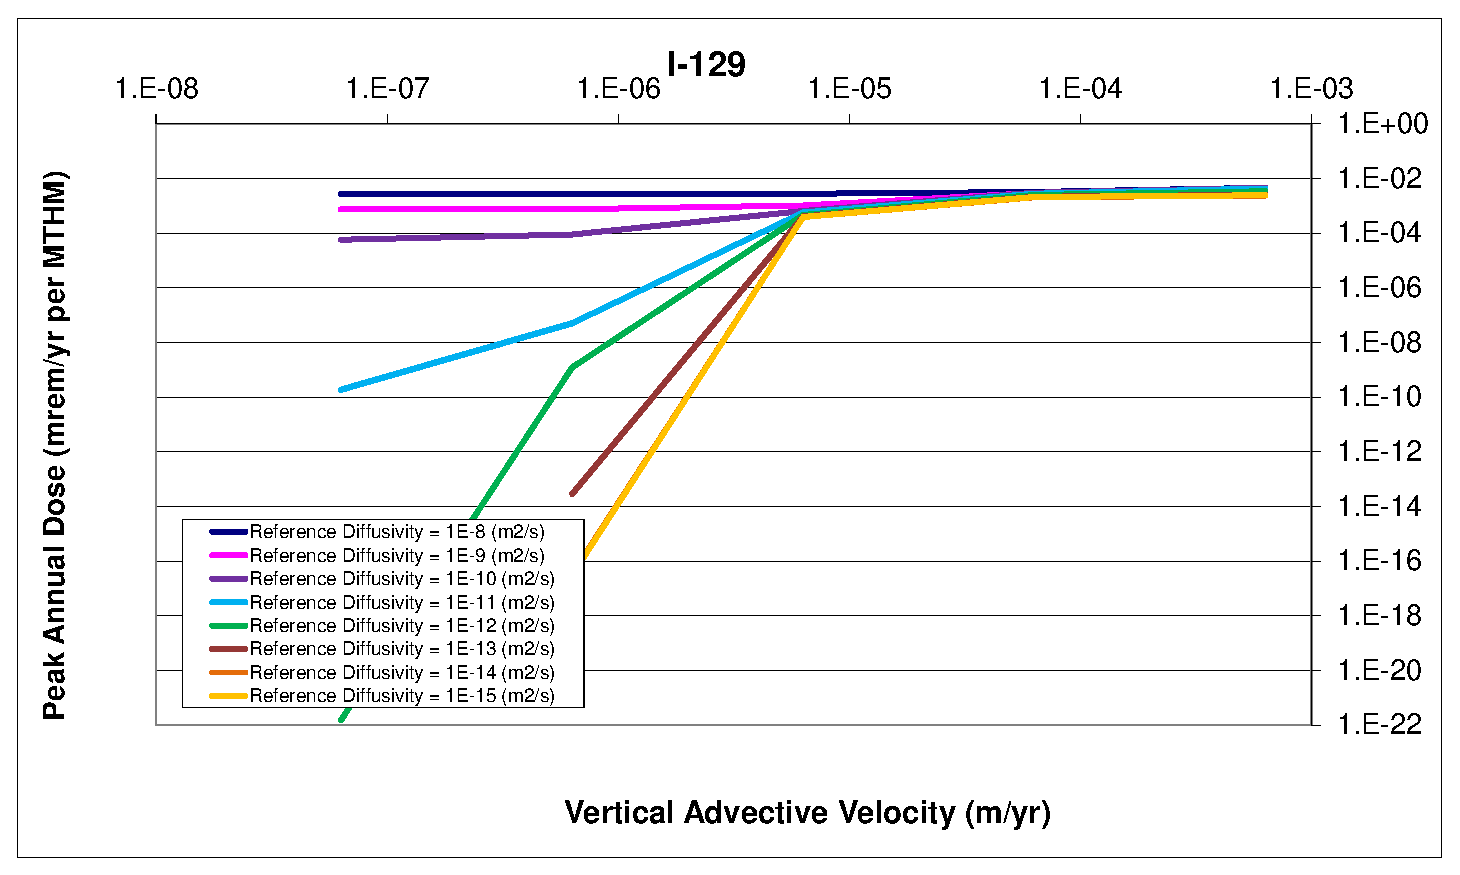
\includegraphics[width=\linewidth]{./nuclide_demonstration/AdvVelDiff/I-129-VAdvVel.eps}
\caption{$^{129}I$ vertical advective velocity sensitivity.}
\label{fig:VAdvVelI129VAdvVel}

\end{minipage}
\end{figure}
\end{frame}


\subsubsection{Advection vs. Diffusion Sensitivity Cyder Results}
Some of the  radionuclide transport models in \Cyder depend on the advective velocity as well as the diffusion 
characteristics of the medium. By evaluating the sensitivity to the advective velocity and reference 
diffusivity of the radionuclide transport in the MixedCell model, trends similar to those found in the \gls{GDSM} were found with the \Cyder tool. 
Specifically, increased advection and increased diffusion lead to greater release. Also, when both are varied, a boundary between diffusive and advective
regimes can be seen. An example of these results are shown in Figure \ref{fig:mixed_adv_diff}.
 
\begin{figure}[ht]
\centering
%\includegraphics[width=\linewidth]{./chapters/demonstration/bench/mixed_diff.eps}
\caption[Advection vs. Diffusion Sensitivity in Cyder]{Dual advective velocity 
and reference diffusivity sensitivity for a non-sorbing, infinitely soluble 
nuclide.}
\label{fig:mixed_adv_diff}
\end{figure}


\FloatBarrier
\subsection{Case II : Solubility Sensitivity}
\begin{frame}[ctb!]
\frametitle{Clay GDSM Solubility Sensitivity}
\begin{figure}[htb!]
\centering
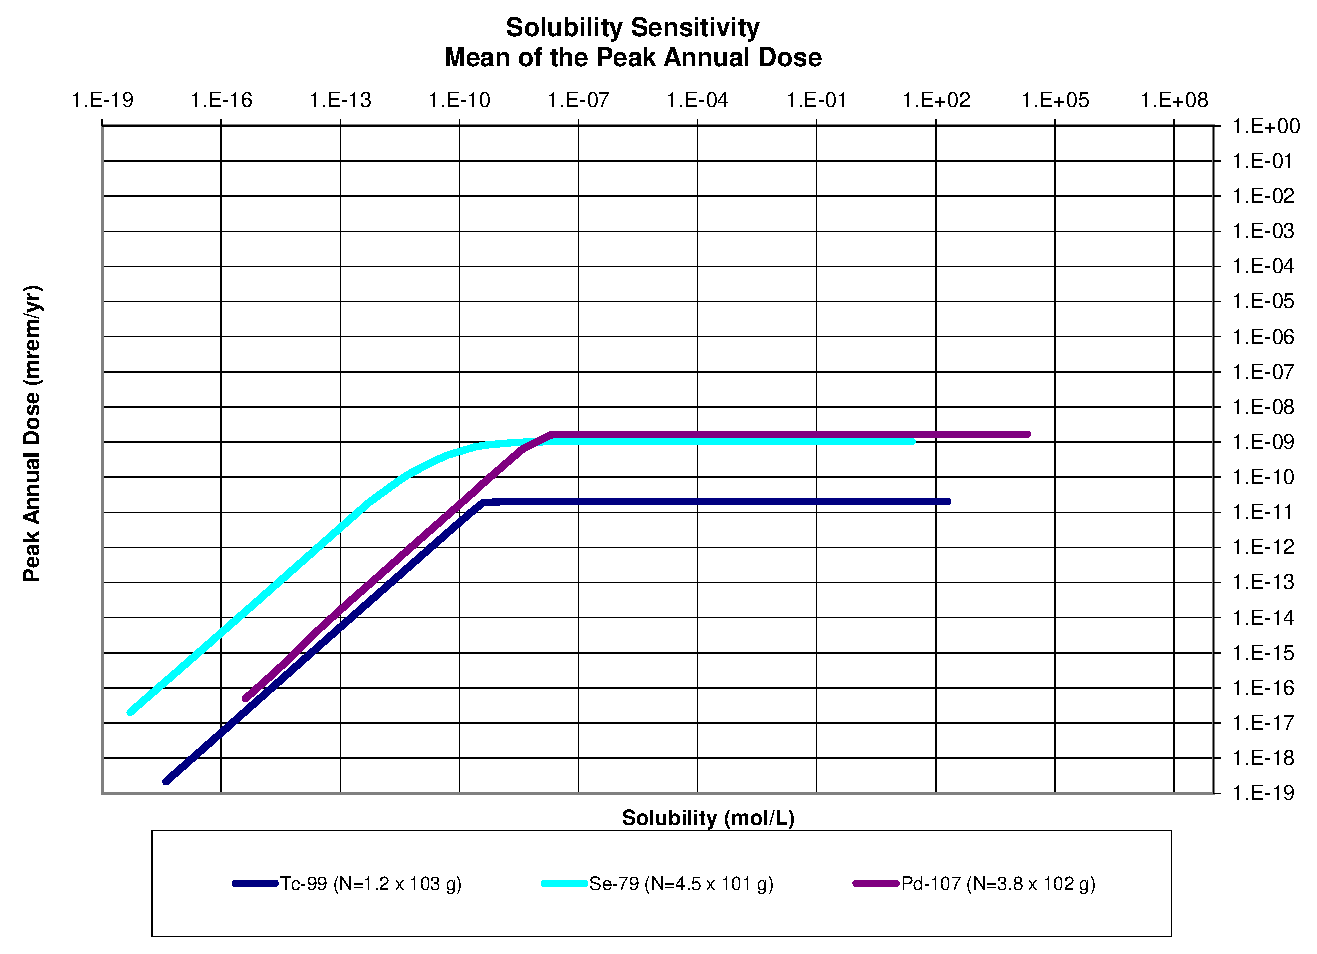
\includegraphics[width=0.7\linewidth]{./nuclide_demonstration/Solubility_Summary_Sol.eps}
\caption{Solubility limit sensitivity. The peak annual dose due to an inventory, 
$N$, of each isotope.}
\label{fig:SolSum}
\end{figure}
\end{frame}

In the parametric analysis of \Cyder performance, it was shown that the 
solubility sensitivity behavior closely matched that of the \gls{GDSM} 
sensitivity behaviors. Specifically, in Figure \ref{fig:sol}.

\begin{figure}[htbp!]
\begin{center}
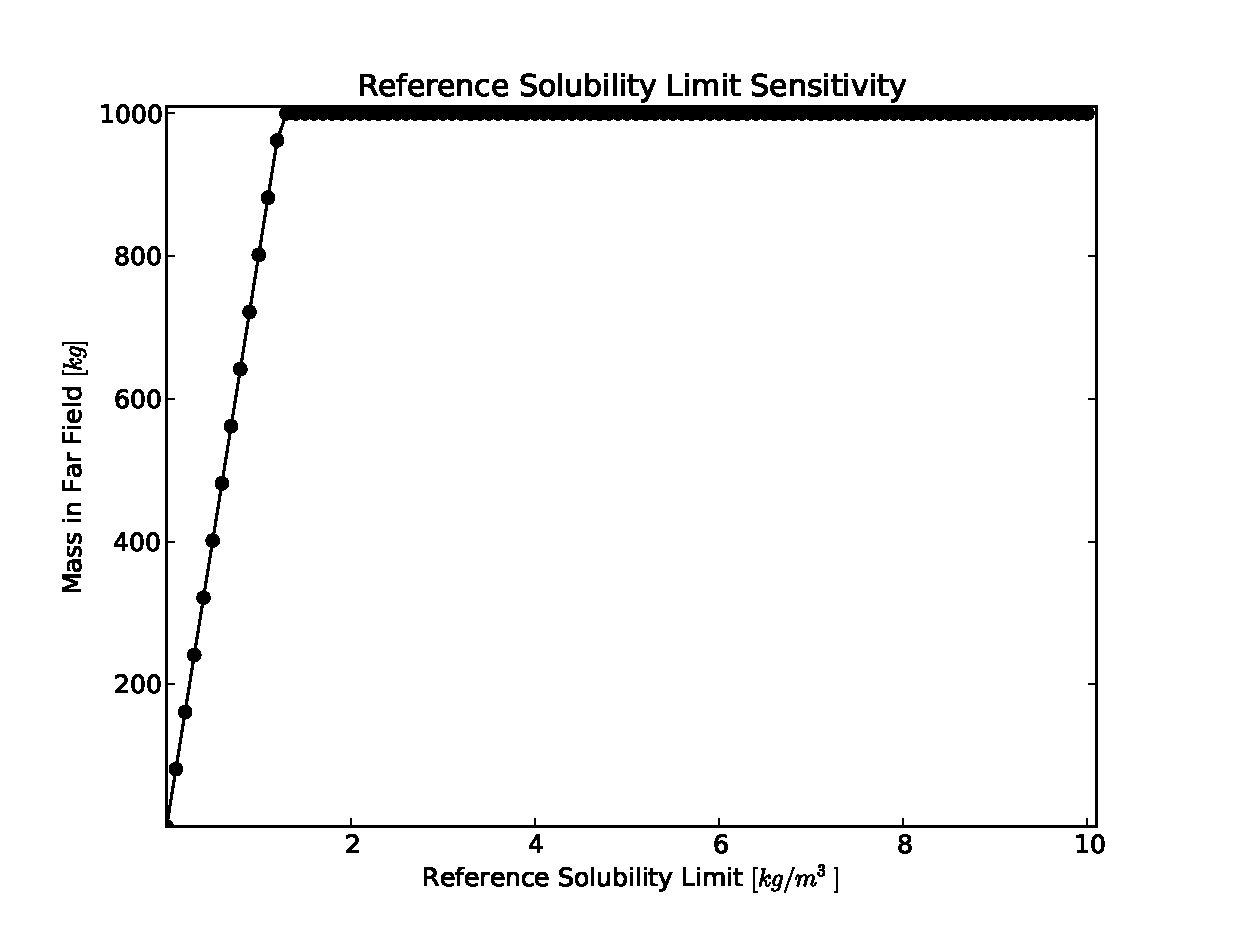
\includegraphics[width=0.8\textwidth]{./chapters/demonstration/bench/sol.eps}
\end{center}
\caption{Sensitivity demonstration of solubility limitation in Cyder for an 
arbitrary isotope assigned a variable solubility limit. }
\label{fig:sol_result}
\end{figure}



\FloatBarrier
\subsection{Case III : Sorption Sensitivity}

\begin{frame}[ctb!]
\frametitle{Clay GDSM Sorption Sensitivity}
\begin{figure}[ht]
\centering
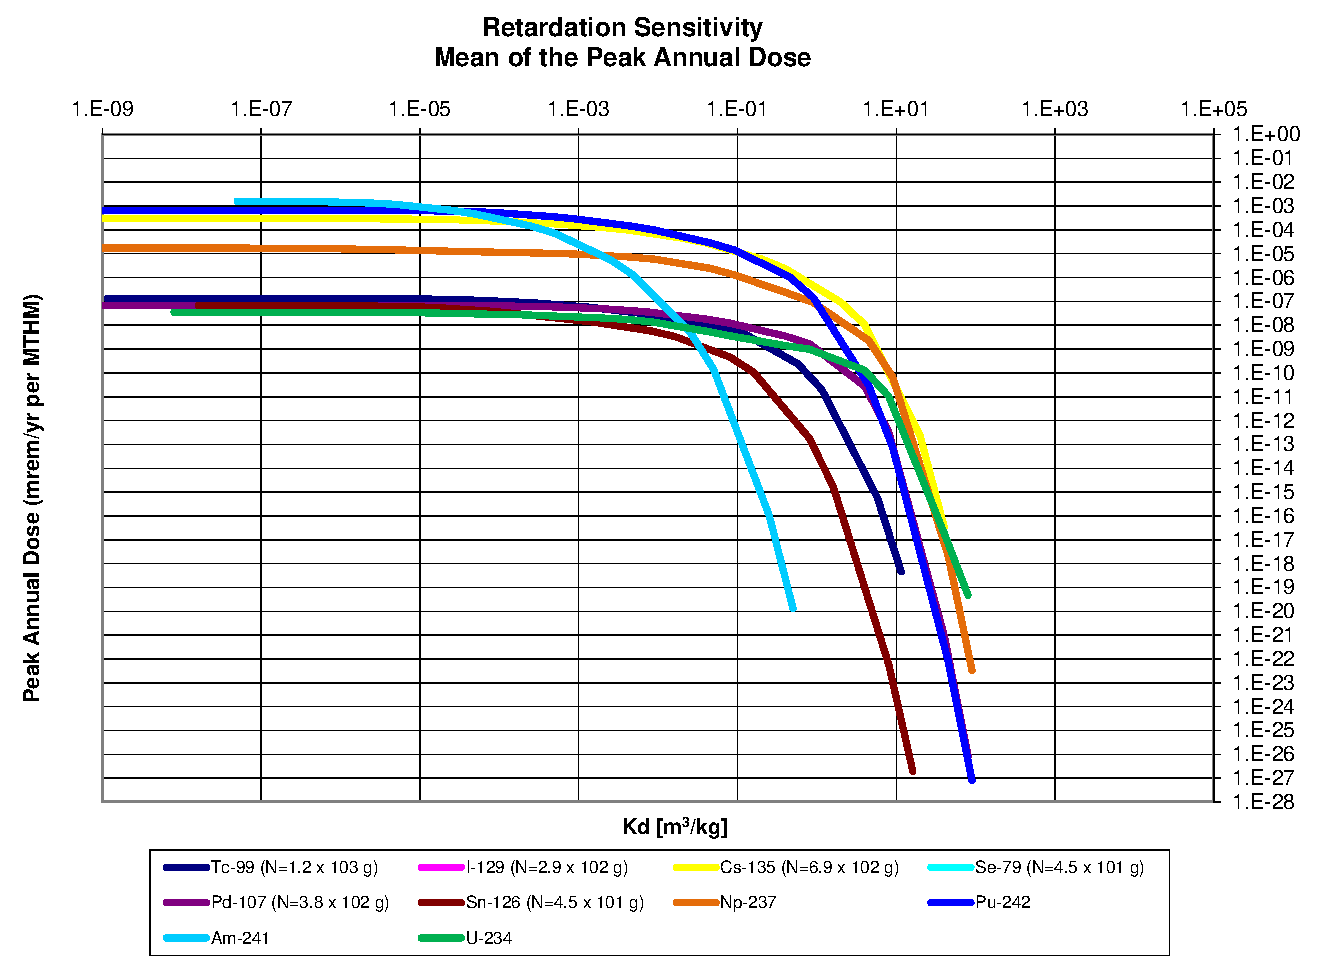
\includegraphics[width=0.7\linewidth]{./nuclide_demonstration/Retardation_Summary_kd.eps}
\caption{$K_d$ sensitivity.  The peak annual dose due to an inventory, 
$N$, of each isotope.}
\label{fig:KdSum}
\end{figure}

\end{frame}


\FloatBarrier
\subsection{Case IV : Waste Form Degradation Rate and Inventory Sensitivity}
\begin{frame}[ctb!]
\frametitle{Clay GDSM Degradation Rate Sensitivity}

\begin{figure}[ht!]
\begin{minipage}[b]{0.45\linewidth}
\centering
\includegraphics[width=\linewidth]{./nuclide_demonstration/DegRate/I-129.eps}
\caption{$^{129}I$ waste form degradation rate sensitivity.}
\label{fig:WFDegI129}

\end{minipage}
\hspace{0.05\linewidth}
\begin{minipage}[b]{0.45\linewidth}

\includegraphics[width=\linewidth]{./nuclide_demonstration/DegRate/I-129-MF.eps}
\caption{$^{129}I$ inventory multiplier sensitivity.}
\label{fig:WFDegI129MF}

\end{minipage}
\end{figure}
\end{frame}

\begin{frame}[ctb]
\frametitle{Cyder Degradation Rate Sensitivity}
In the parametric sensitivity analysis conducted with the \Cyder tool, waste 
form degradation rate sensitvity similarly shows the two regimes noted in the 
GDSM analysis.  


\begin{figure}[htbp!]
\begin{center}
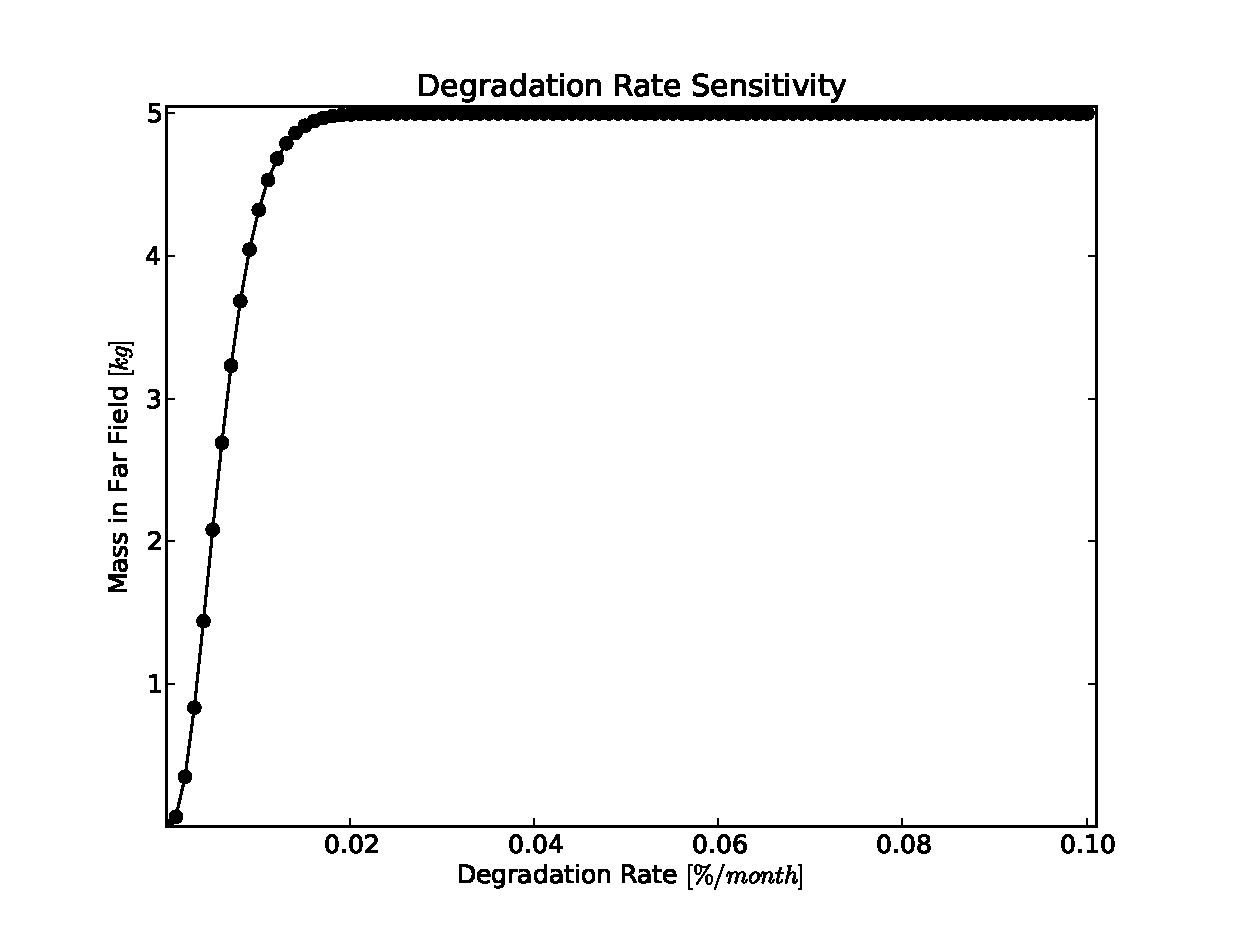
\includegraphics[width=0.7\linewidth]{./nuclide_demonstration/deg.eps}
\end{center}
\caption{Sensitivity demonstration of the degradation rate in \Cyder for an 
arbitrary isotope.}
\label{fig:deg}
\end{figure}
\end{frame}


%\subsection{Case IVI : Waste Package Failure Time and Diffusion Coefficient Sensitivity}
%\subsubsection{Waste Package Failure Time Sensitivity}

In the parametric sensitivity analysis discussed in Section 
\ref{sec:wpfail}, it was shown that For the clay repository, the waste 
package failure time is entirely irrelevant until waste package failure times 
reach the million or ten million year time scale. 

\begin{figure}[ht!]
  \centering
  \begin{minipage}[b]{0.45\linewidth}
    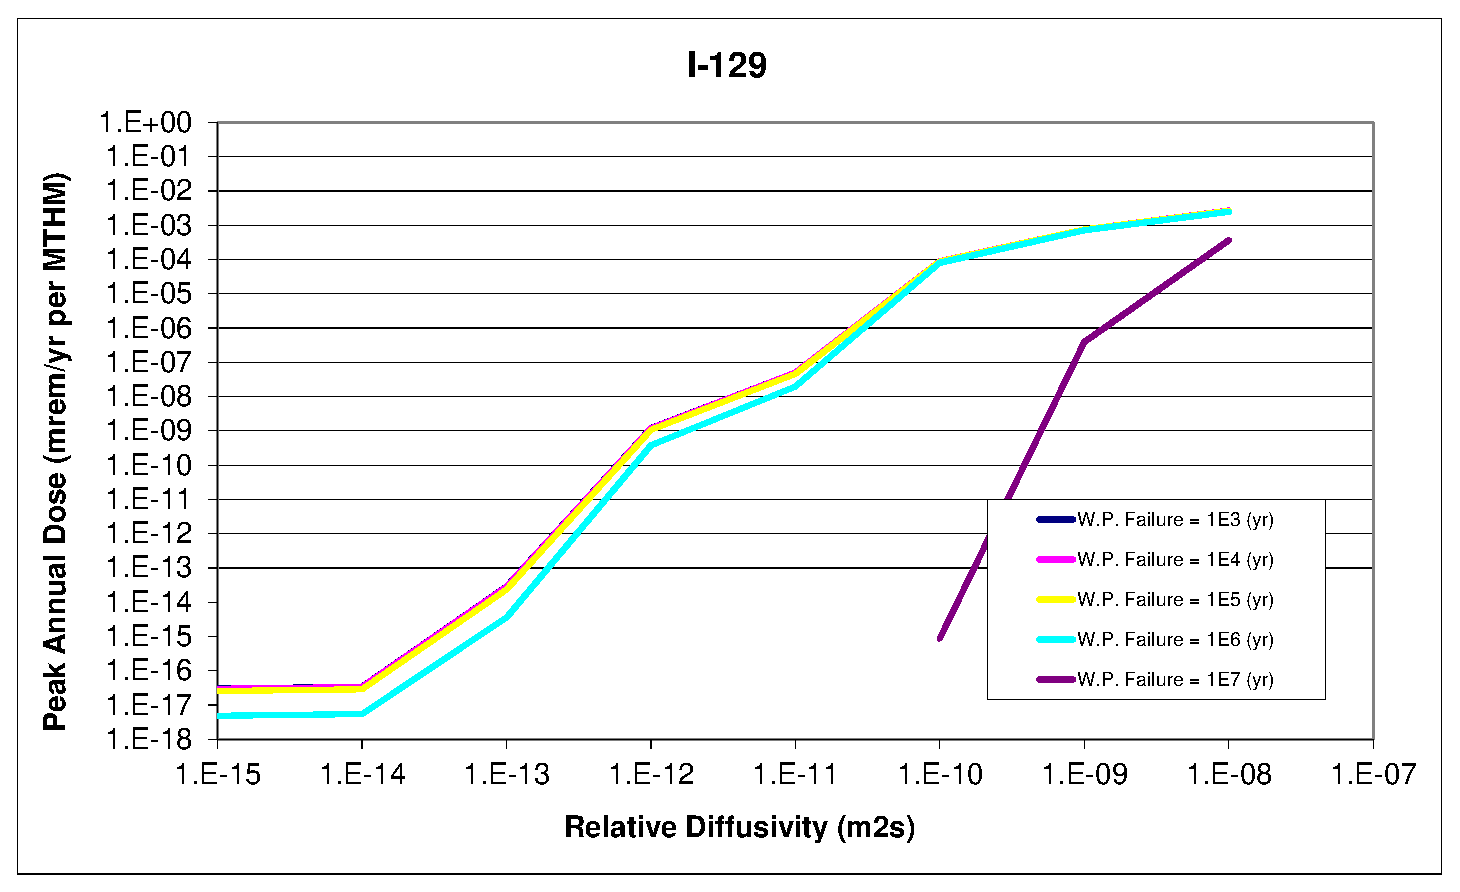
\includegraphics[width=\linewidth]{./chapters/nuclide_sensitivity/clay/WPFailExtended/I-129.eps}
    \caption{$^{129}I$ waste package failure time sensitivity. }
    \label{fig:WPFailI129}

  \end{minipage}
  \hspace{0.05\linewidth}
  \begin{minipage}[b]{0.45\linewidth}

    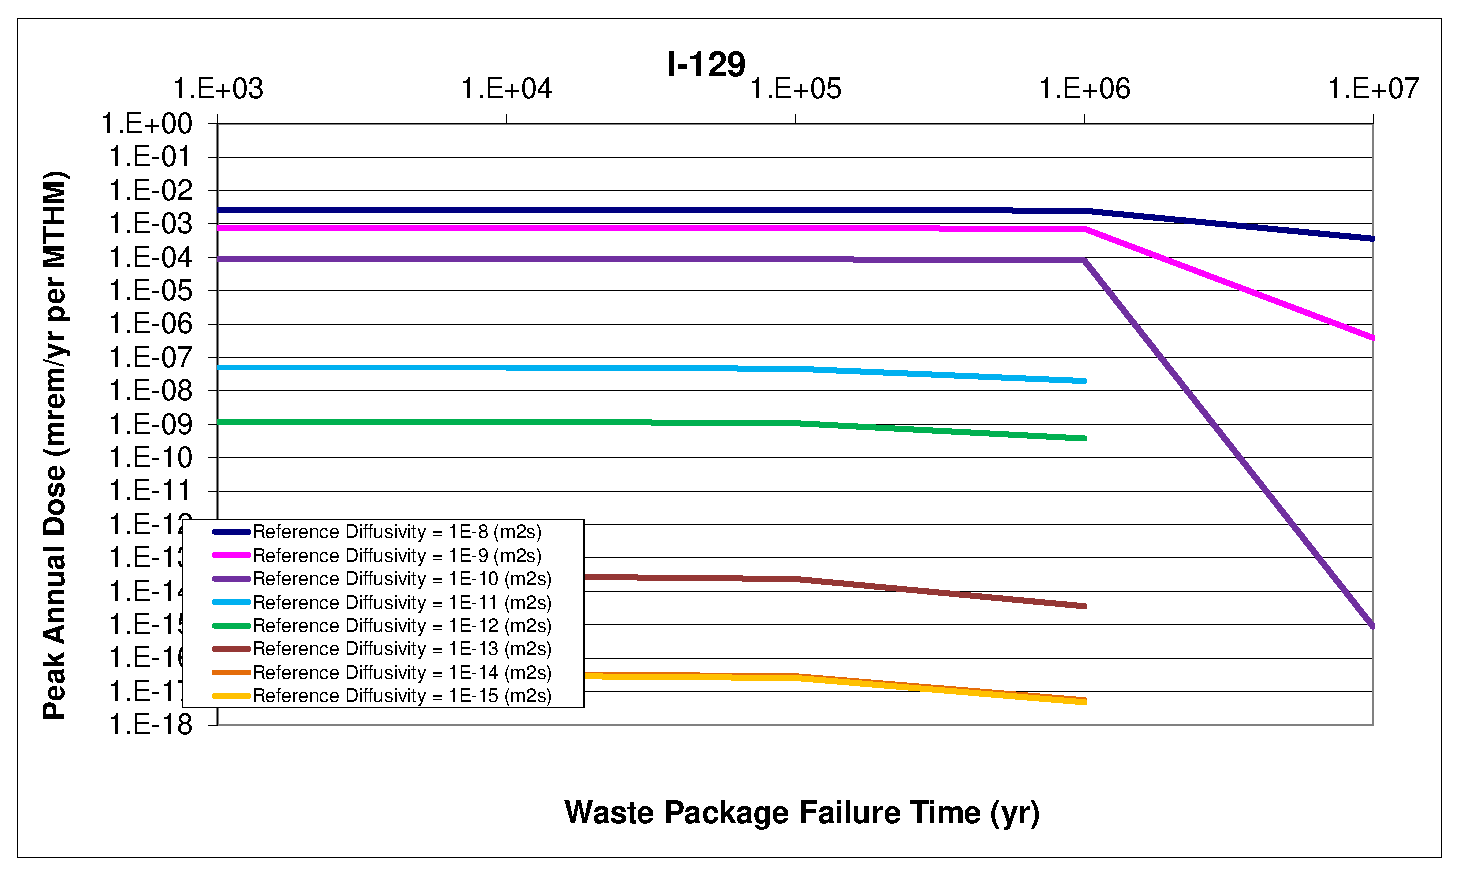
\includegraphics[width=\linewidth]{./chapters/nuclide_sensitivity/clay/WPFailExtended/I-129-WPFail.eps}
    \caption{$^{129}I$ waste package failure time sensitivity. }
    \label{fig:WPFailI129}

  \end{minipage}
\end{figure}
\begin{figure}[ht]
  \begin{minipage}[b]{0.45\linewidth}

    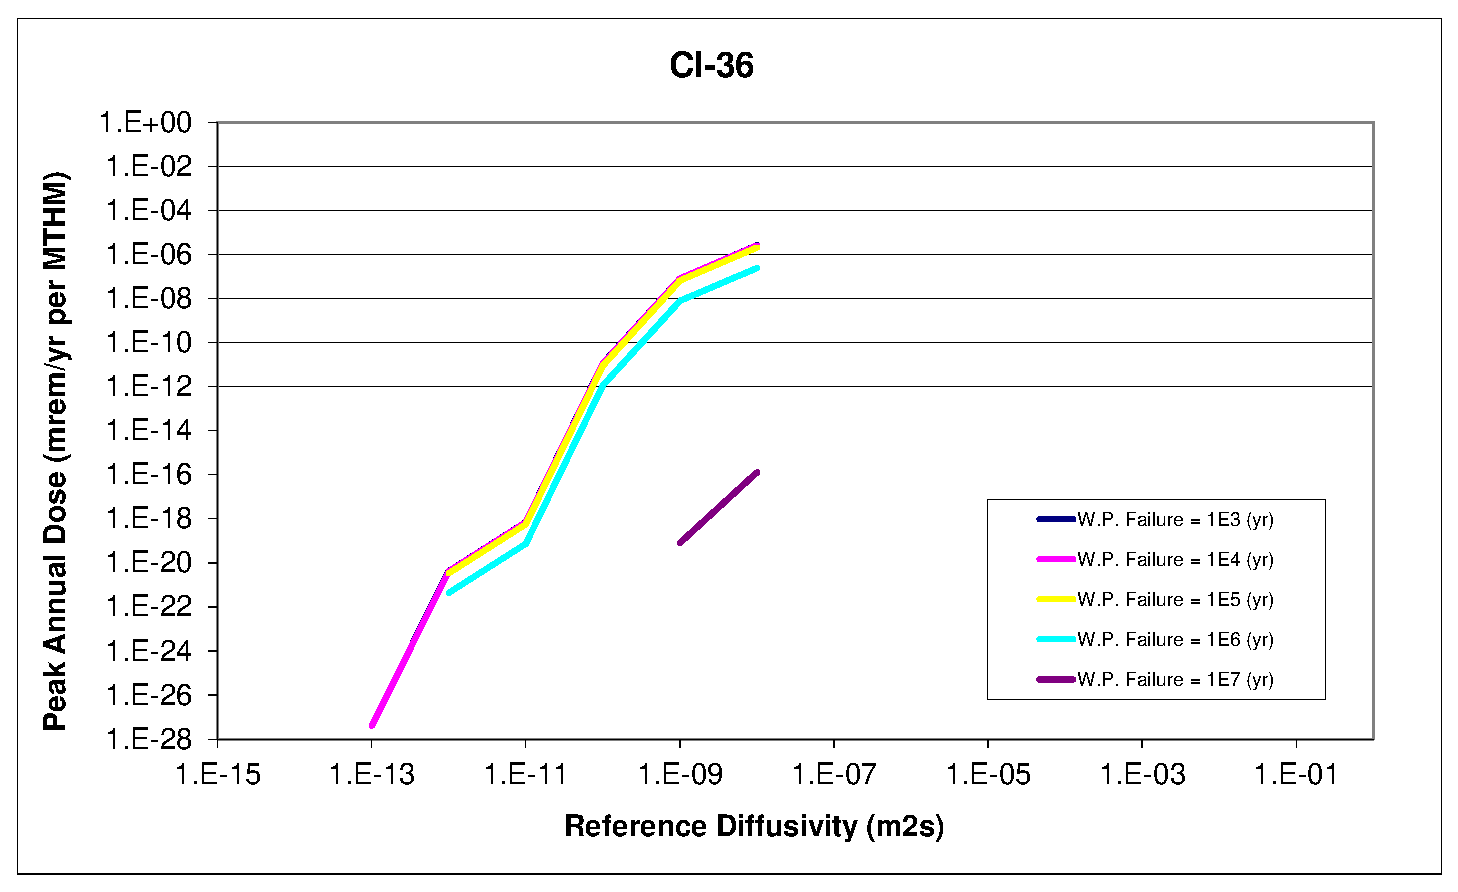
\includegraphics[width=\linewidth]{./chapters/nuclide_sensitivity/clay/WPFailExtended/Cl-36.eps}
    \caption{$^{36}Cl$ waste package failure time sensitivity. }
    \label{fig:WPFailCl36}

  \end{minipage}
  \hspace{0.05\linewidth}
  \begin{minipage}[b]{0.45\linewidth}

    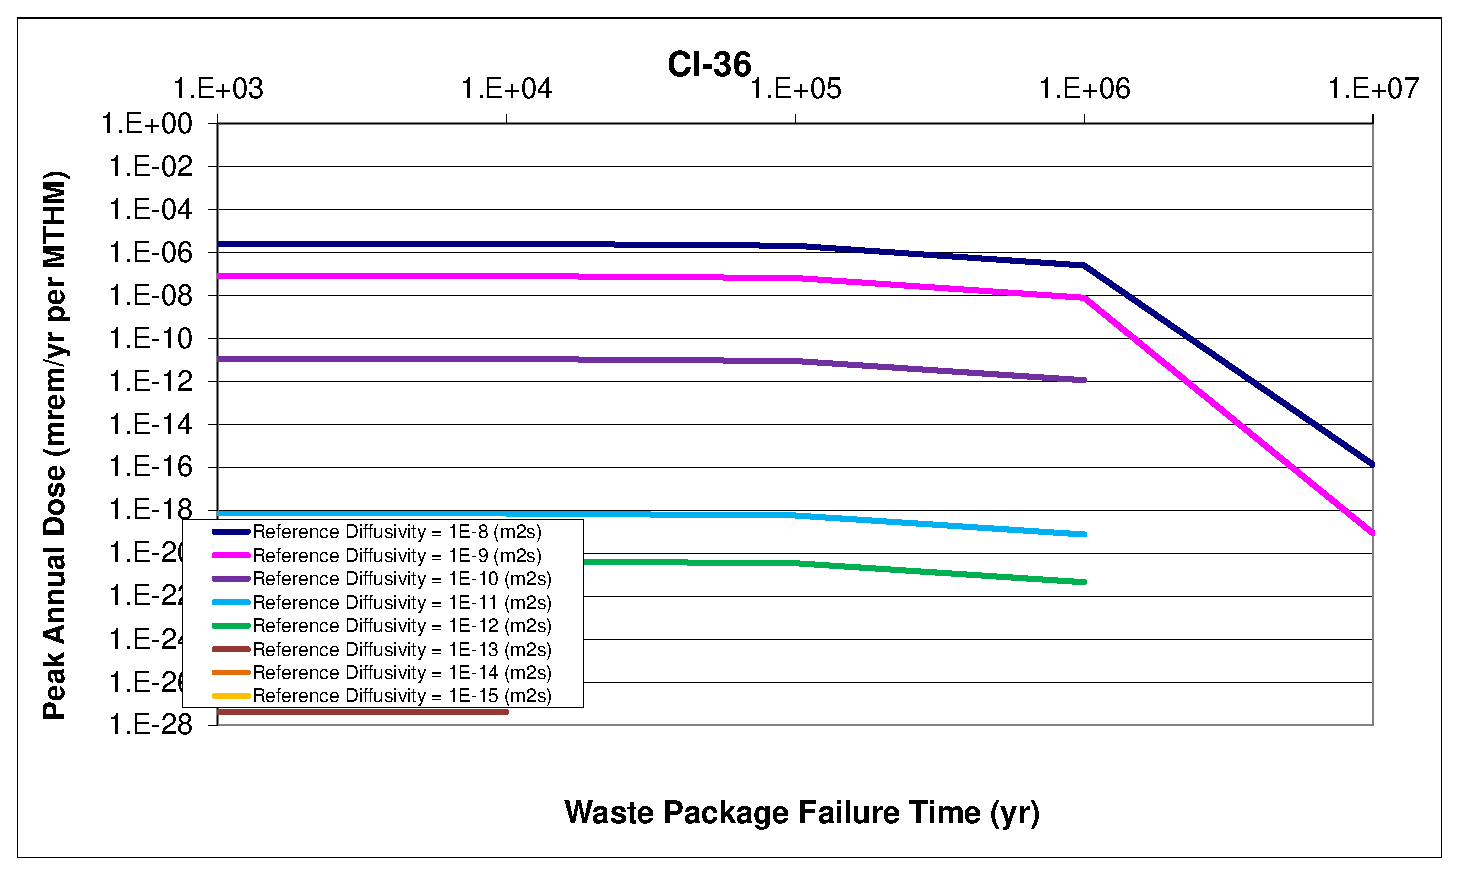
\includegraphics[width=\linewidth]{./chapters/nuclide_sensitivity/clay/WPFailExtended/Cl-36-WPFail.eps}
    \caption{$^{36}Cl$ waste package failure time sensitivity. }
    \label{fig:WPFailPuDaughters}

  \end{minipage}
\end{figure}


\begin{figure}[ht!]
  \centering
  \begin{minipage}[b]{0.45\linewidth}

    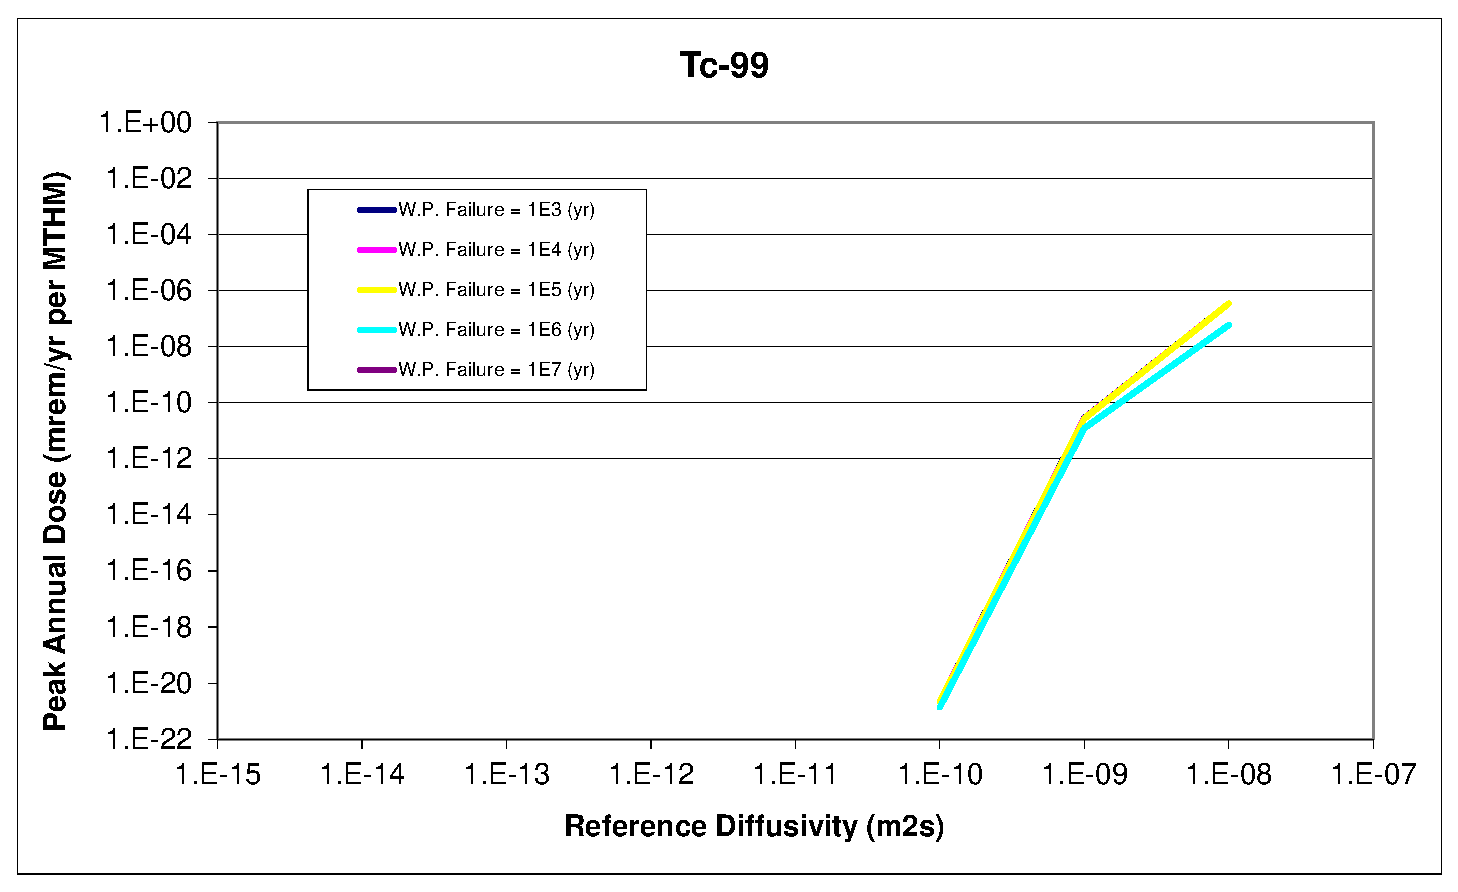
\includegraphics[width=\linewidth]{./chapters/nuclide_sensitivity/clay/WPFailExtended/Tc-99.eps}
    \caption{$^{99}Tc$ waste package failure time sensitivity. }
    \label{fig:WPFailTc99}

  \end{minipage}
  \hspace{0.05\linewidth}
  \begin{minipage}[b]{0.45\linewidth}

    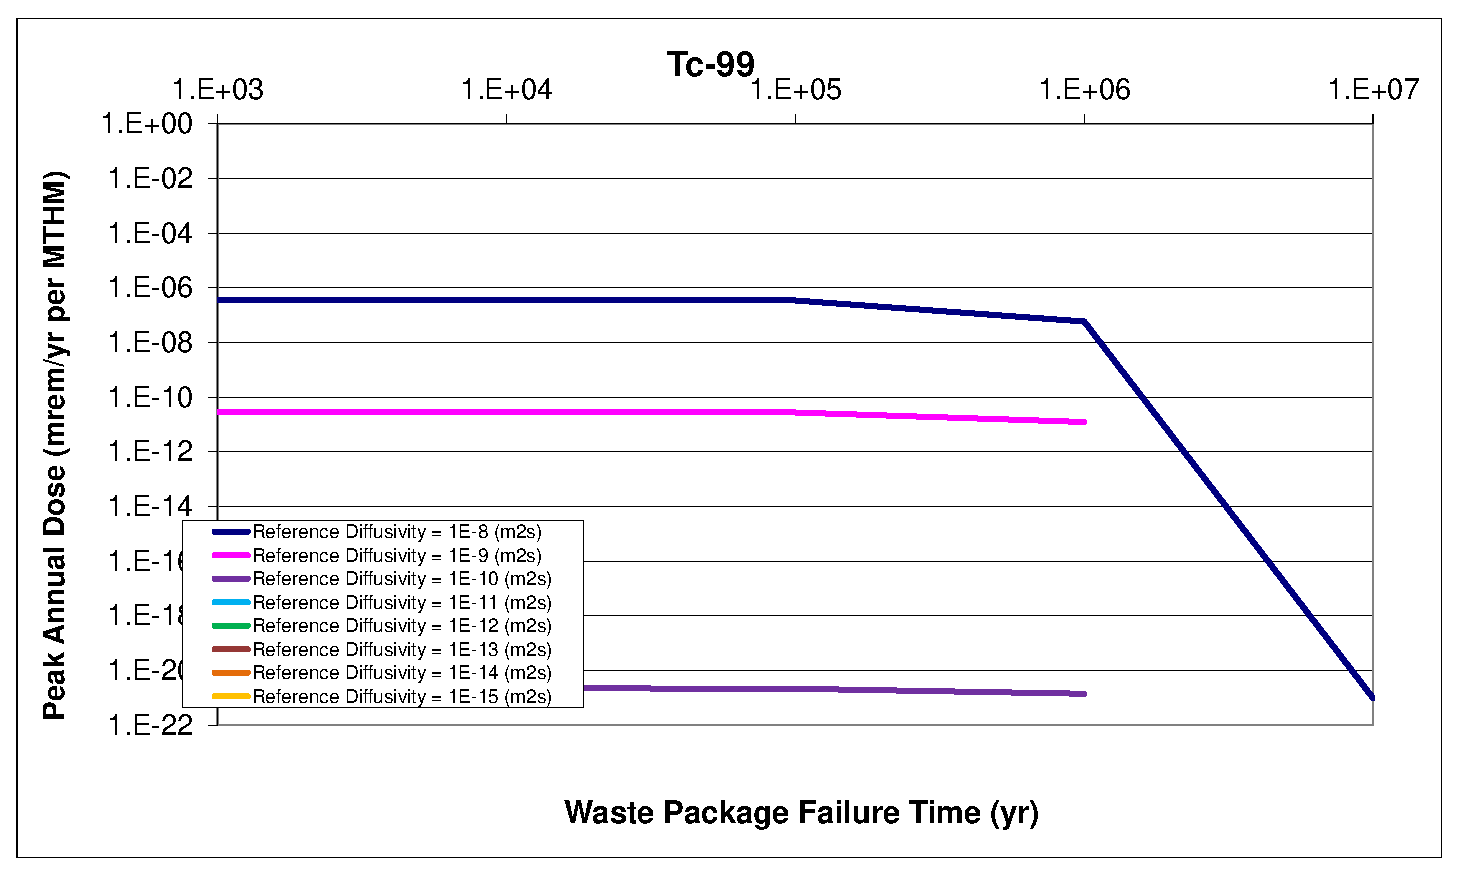
\includegraphics[width=\linewidth]{./chapters/nuclide_sensitivity/clay/WPFailExtended/Tc-99-WPFail.eps}
    \caption{$^{99}Tc$ waste package failure time sensitivity. }
    \label{fig:WPFailTc99}

  \end{minipage}
\end{figure}
\begin{figure}[ht]
  \begin{minipage}[b]{0.45\linewidth}

    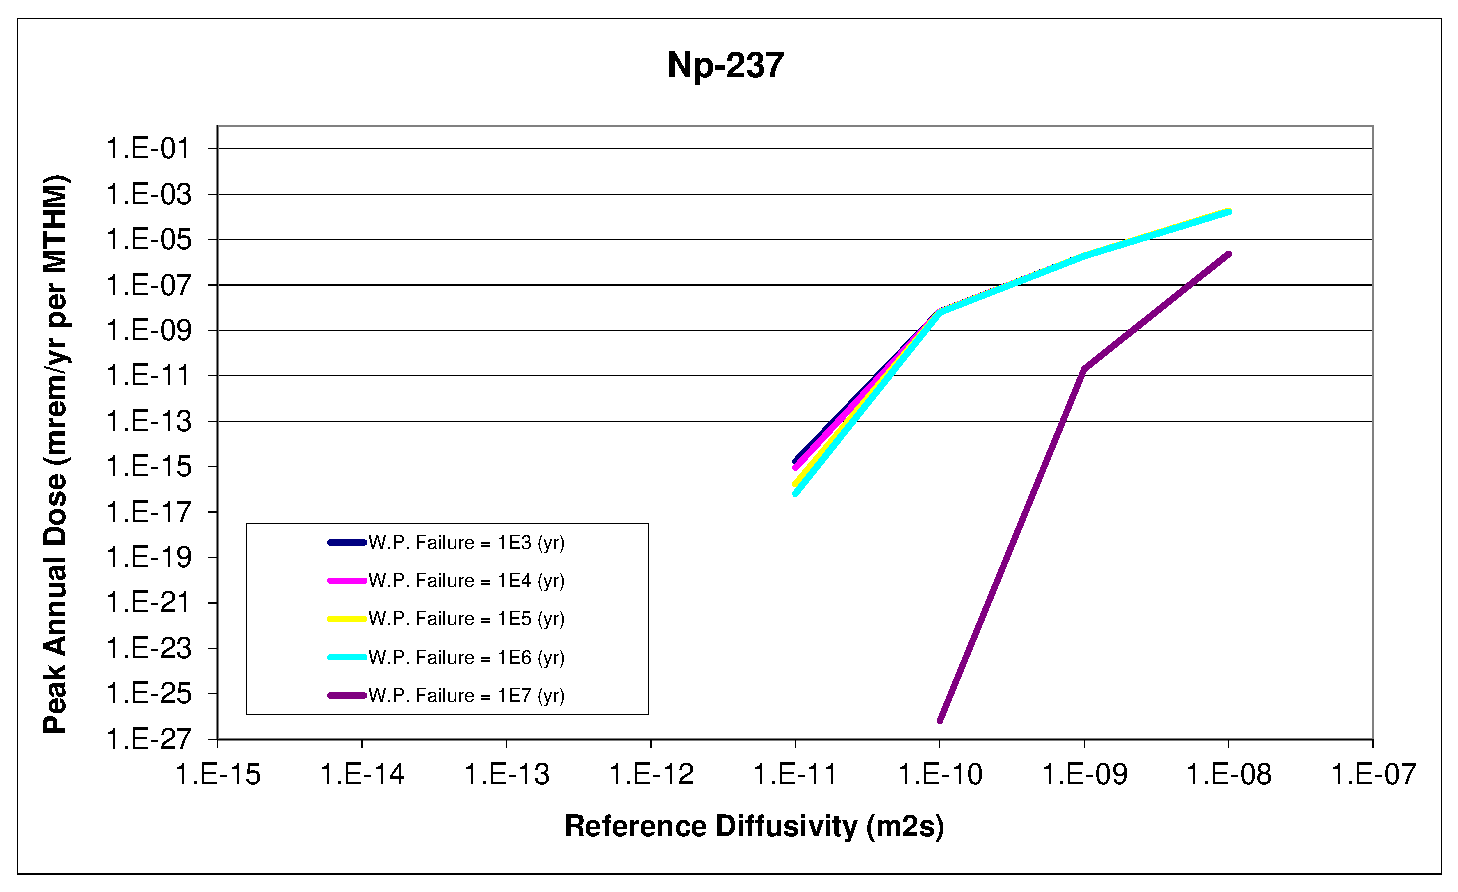
\includegraphics[width=\linewidth]{./chapters/nuclide_sensitivity/clay/WPFailExtended/Np-237.eps}
    \caption{$^{237}Np$ waste package failure time sensitivity. }
    \label{fig:WPFailNp237}

  \end{minipage}
  \hspace{0.05\linewidth}
  \begin{minipage}[b]{0.45\linewidth}

    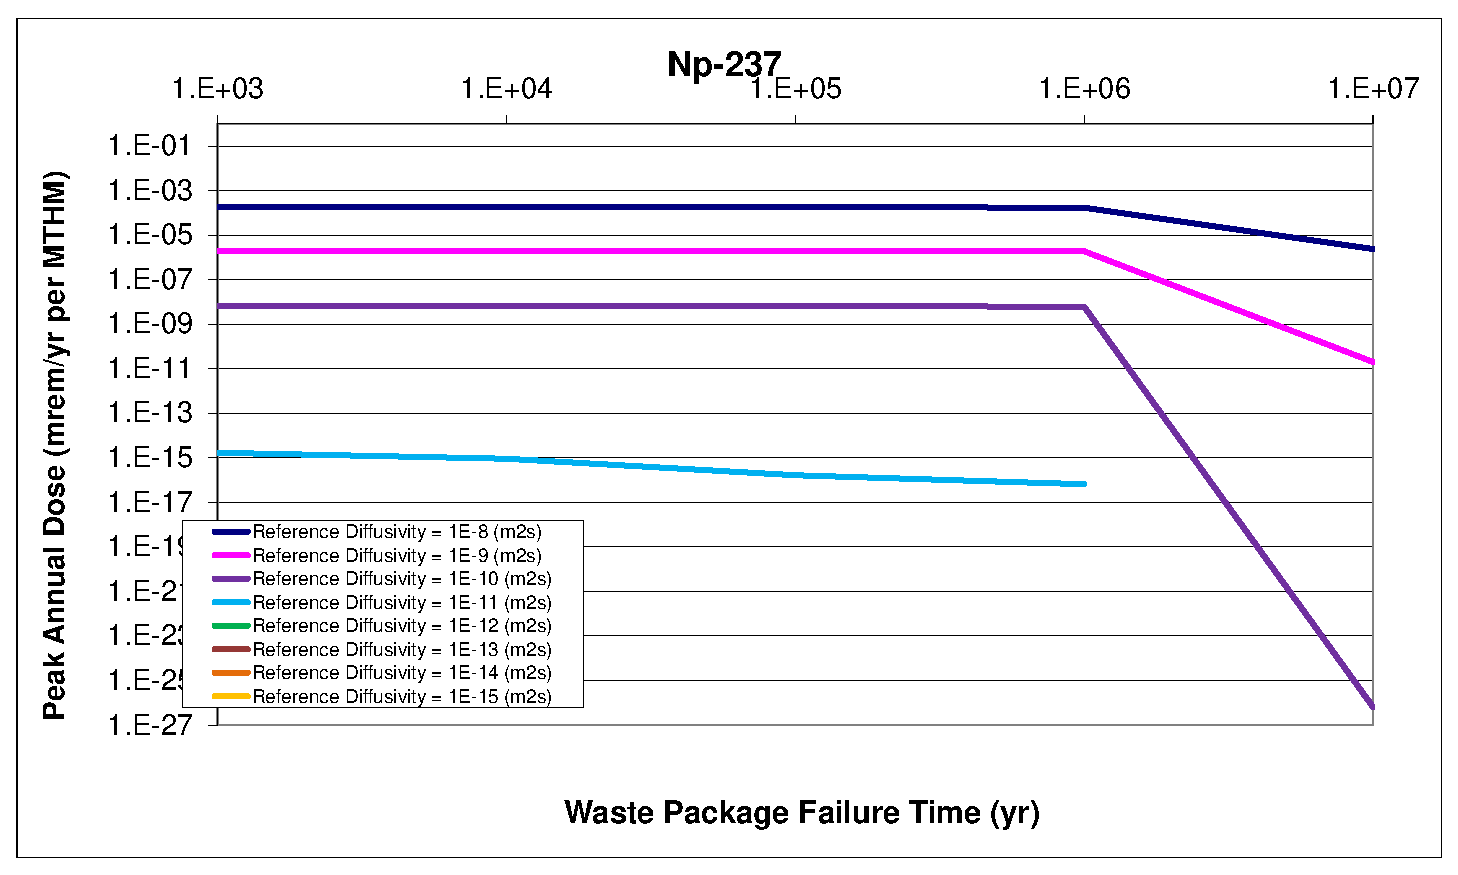
\includegraphics[width=\linewidth]{./chapters/nuclide_sensitivity/clay/WPFailExtended/Np-237-WPFail.eps}
    \caption{$^{237}Np$ waste package failure time sensitivity. }
    \label{fig:WPFailPuDaughters}

  \end{minipage}
\end{figure}

\clearpage



\FloatBarrier
